\documentclass{article}
\usepackage[utf8]{inputenc}
\usepackage[russian]{babel}
\usepackage{graphicx}
\usepackage{caption}
\usepackage{float}
\usepackage{hyperref}
\usepackage{xcolor}
\usepackage[unicode, pdftex]{hyperref}
\usepackage[left=2cm,right=2cm,top=2cm,bottom=2cm,bindingoffset=0cm]{geometry}
    
\graphicspath{{pictures/}}
\DeclareGraphicsExtensions{.pdf,.png,.jpg}
\definecolor{urlcolor}{HTML}{003bed}

\hypersetup{pdfstartview=FitH, linkcolor=linkcolor,urlcolor=urlcolor, colorlinks=true}

\begin{document}
    % ТИТУЛЬНИК
    \begin{center}
        \hfill \break
        \LARGE{Дискретная математика}\\
        \hfill \break
        \Large{Домашняя работа 6}\\
        \hfill \break
        \hfill \break
        \hfill \break
        \hfill \break
    \end{center}

    \begin{flushright} Ученик: Титов Даниил, M3104 \end{flushright}
    \begin{flushright} Преподаватель: Lipenx \end{flushright}
    \vfill
    \bigskip
    \begin{center} Санкт-Петербург \end{center}
    \begin{center} 2021 \end{center}
    \thispagestyle{empty}
    \newpage
    % СОДЕРЖАНИЕ
    \tableofcontents{}
    \newpage
    % РЕШЕНИЯ
    \section{Найдите количество различных 5-значных чисел, используя цифры 1-9 при заданных ограничениях. Для каждого случая приведите несколько примеров соответствующих чисел и выведите общую формулу}
        \subsection{Цифры могут повторяться}
            Так как цифры могут повторяться, то на 1ую позицию у нас есть 9 цифр, на 2ую тоже, на 3-5ые аналогично\\
            \textit{Общая формула:} $ \overline{A^k_n} = n^k = 9*9*9*9*9 = 9^5 $\\
            \textit{Пример чисел:}\\
            - $11111$\\
            - $22223$\\
            - $96185$
        \subsection{Цифры не могут повторяться}
            Так как цифры не могут повторяться, то на 1ую позицию у нас есть 9 цифр, на 2ую 8, на 3ью 7 и так далее\\
            \textit{Общая формула:} $ A^k_n = \frac{n!}{(n-k)!} = \frac{9!}{(9-5)!} = 9*8*7*6*5 = 15120 $\\
            \textit{Пример чисел:}\\
            - 12345\\
            - 29476\\
            - 97842
        \hypertarget{1c}{\subsection{Цифры могут повторяться и должны быть записаны в невозрастающем порядке}}
            В данной задаче мы будем использовать Stars and Bars, и исходя из этого\\
            \textit{Общая формула:} $ C^{n-1}_{n+k-1} = \frac{(n+k-1)!}{(n-1)!*((n+k-1)-(n-1))!} = \frac{13!}{8!*(13-8)!} = 1287 $\\
            \textit{Пример чисел:}\\
            - $98765 - ||||*|*|*|*|*$\\
            - $99887 - ||||||*|**|**$\\
            - $76541 - *|||*|*|*|*||$
        \subsection{Цифры не могут повторяться и должны быть записаны в порядке возрастания}
            Чтобы понять, сколько чисел нам нужно взять, возьмём любое 5-значное число, например, 92134. Надо, чтобы цифры в нём шли по возрастанию и оно однозначно становится таким: 12349, и так у нас будет всегда, следовательно существует лишь одно число из выборки, цифры которого идут в порядке возрастания\\
            \textit{Общая формула:} $ C^n_k = \frac{n!}{k!*(n-k)} = \frac{9!}{5!*(9-5)!} = 126 $\\
            \textit{Пример чисел:}\\
            - 12345\\
            - 23456\\
            - 56789
        \subsection{Цифры могут повторяться, должны быть записаны в неубывающем порядке, а 4-я цифра должна быть 6}
            Я бы разбил данную задачу на две подзадачи, так как у нас есть 4-я цифра, которая точно должна быть 6 + условие о неубывающем порядке, следовательно:\\\\
            1. Первые три цифры могут быть от 1 до 6 включительно, строго в неубывающем порядке, то есть наша задача \hyperlink{1c}{1.3}, то есть для первых трёх чисел будет:\\
            $ C^{n-1}_{n+k-1} = \frac{(n+k-1)!}{(n-1)!*((n+k-1)-(n-1))!} $, где $ n - 6 $, а $ k - 3 $, следовательно:\\
            $ C^{5}_{8} = \frac{8!}{5!*(8-5)!} = 56 $\\
            2. Четвёртая цифра нам известна - 6, значит остаётся пятая, из-за условия о неубывании она может быть 6-9, следовательно это 4 случая\\\\
            Итого: объединив 2 подзадачи, мы получаем $ 56*4 $ случаев, то есть 224\\\\
            \textit{Общая формула:} $ C^{n-1}_{n+k-1} * 4 = \frac{(n+k-1)!}{(n-1)!*((n+k-1)-(n-1))!} * 4 = C^{5}_{8} * 4 = \frac{8!}{5!*(8-5)!} * 4 = 56 * 4 = 224 $\\
            \textit{Пример чисел:}\\
            - 11166\\
            - 12367\\
            - 15679
    \newpage
    \section{Одной из классических комбинаторных задач является подсчет количества расположений $n$ шариков в $k$ коробках. Существует по крайней мере 12 вариантов этой проблемы: четыре случая (a–d) с тремя различными ограничениями (1-3). Для каждой задачи (случай+ограничение) выведите соответствующую общую формулу. Кроме того, выберите несколько (репрезентативных) значений для $n$ и $k$ и используйте полученные формулы для поиска чисел аранжировок, чтобы визуализировать несколько возможных аранжировок для выбранных $n$ и $k$}
        \subsection{U → L: Шары не помечены, Коробки помечены}
            \subsubsection{$\le$ 1 мяч на коробку}
                Так как нам нужно выбрать Коробки, которые мы заполняем одним Шаром, то:\\
                \textit{Общая формула:} $ C^n_k = \frac{k!}{n!*(k-n)!} $\\
                \textit{Пример 1:} $ C^3_2 $ - невозможно, так как Шаров больше, чем Коробок - 0
                \begin{figure}[h!]
                    \fbox{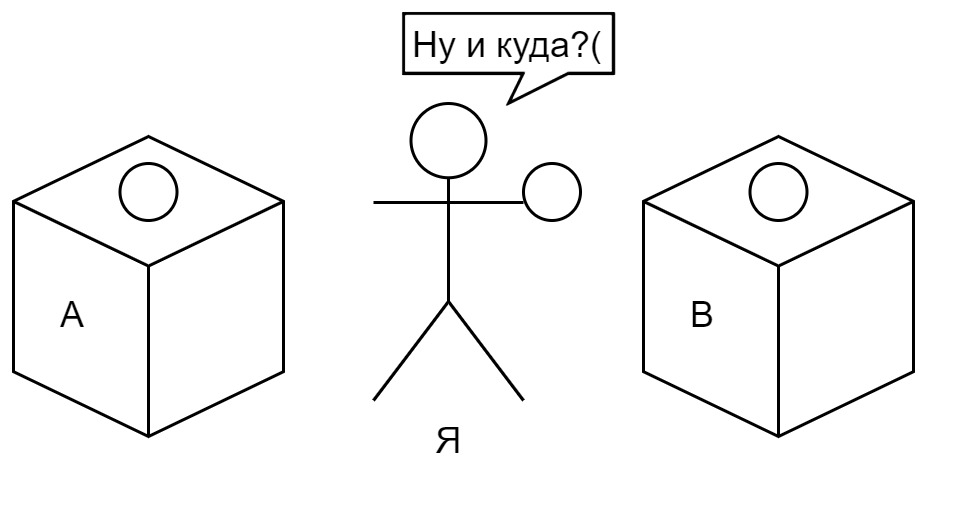
\includegraphics[scale=0.1]{a11.jpg}}
                \end{figure}\\
                \textit{Пример 2:} $ C^4_4 = 1 $
                \begin{figure}[h!]
                    \fbox{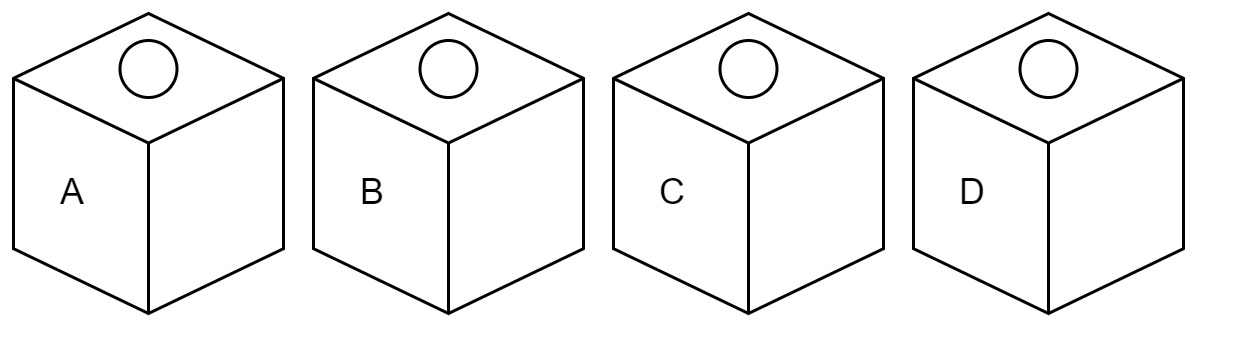
\includegraphics[scale=0.1]{a12.jpg}}
                \end{figure}
            \subsubsection{$\ge$ 1 мяч в коробке}
                Будем использовать метод "Stars and Bars"\\
                Чтобы разбить $n$ Шаров на $k$ Коробок нам понадобится $k-1$ перегородок и $n-1$ мест для них, следовательно:\\
                \textit{Общая формула:} $ C^{k-1}_{n-1} = \frac{(n-1)!}{(k-1)!*((n-1)-(k-1))!} = \frac{(n-1)!}{(k-1)!*(n-k)!} $\\
                \textit{Пример 1:} $ C^{4-1}_{10-1} = 84 $
                \begin{figure}[h!]
                    \fbox{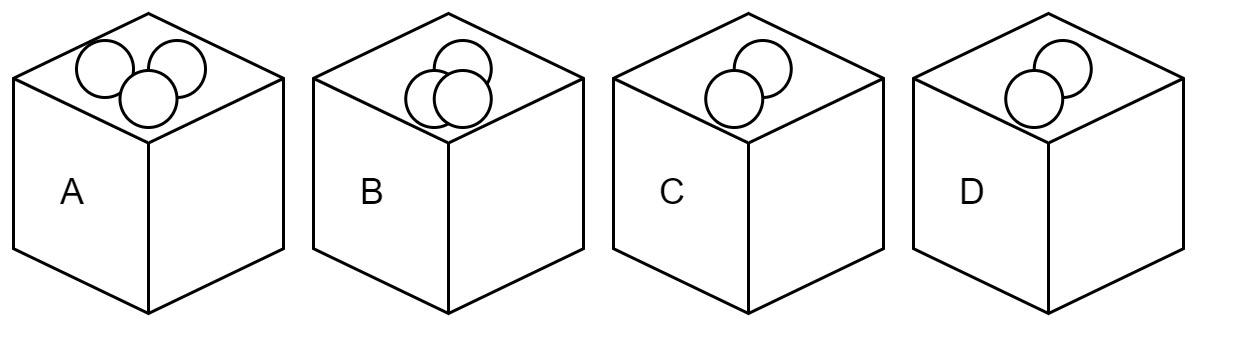
\includegraphics[scale=0.1]{a21.jpg}}
                \end{figure}\\
                \textit{Пример 2:} $ C^{4-1}_{4-1} = 1 $
                \begin{figure}[h!]
                    \fbox{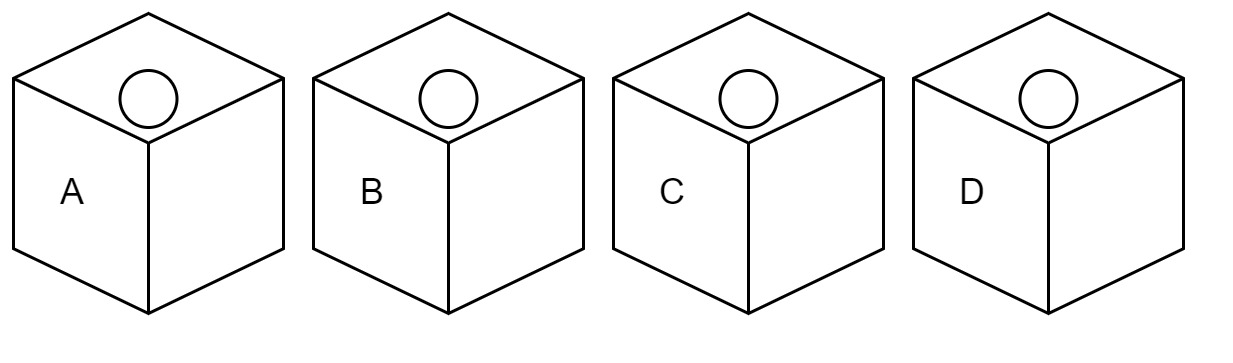
\includegraphics[scale=0.1]{a22.jpg}}
                \end{figure}
            \subsubsection{Произвольное количество шаров в коробке}
                Будем использовать метод "Stars and Bars"\\
                Чтобы разбить $n$ Шаров на $k$ Коробок нам понадобится $k-1$ перегородок и $n+k-1$ мест для них, следовательно:\\
                \textit{Общая формула:} $ C^{k-1}_{n+k-1} = \frac{(n+k-1)!}{(k-1)!*((n+k-1)-(k-1))!} = \frac{(n+k-1)!}{(k-1)!*n!} $\\
                \textit{Пример 1:} $ C^{4-1}_{4+4-1} = 1 $
                \begin{figure}[h!]
                    \fbox{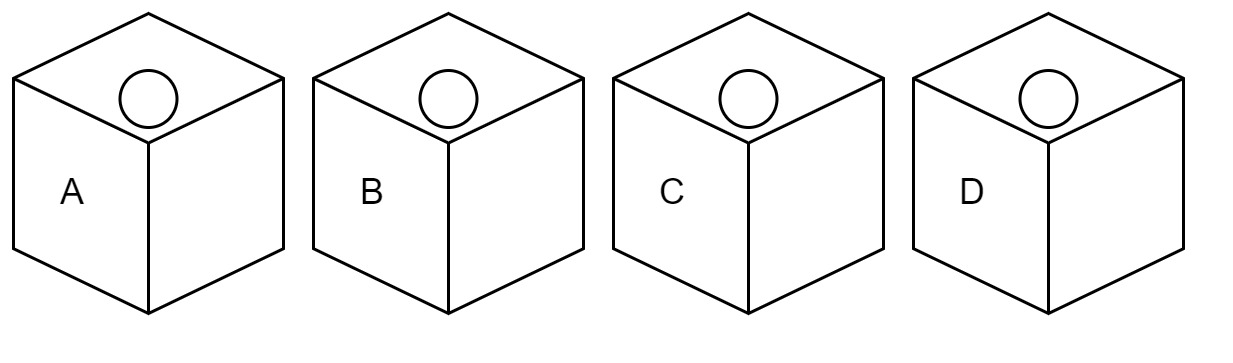
\includegraphics[scale=0.1]{a31.jpg}}
                \end{figure}\\
                \textit{Пример 2:} $ C^{4-1}_{2+4-1} = 10 $
                \begin{figure}[h!]
                    \fbox{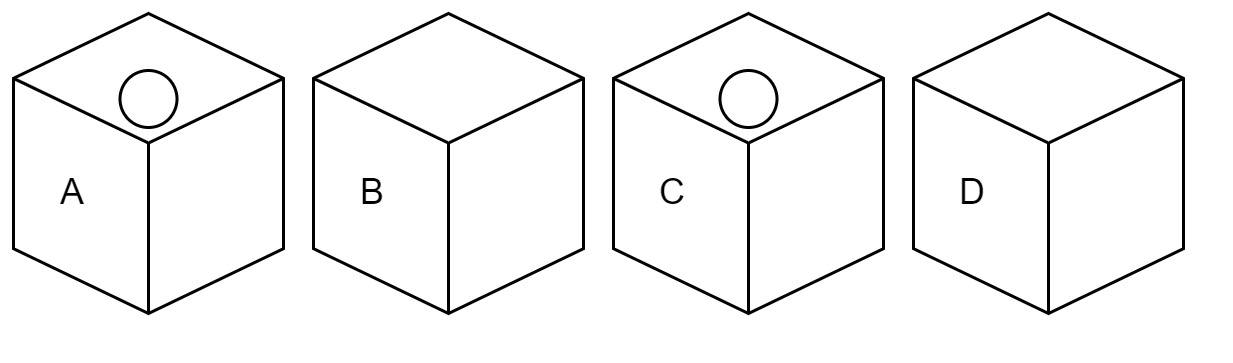
\includegraphics[scale=0.1]{a32.jpg}}
                \end{figure}
        \subsection{L → U: Шары помечены, Коробки не помечены}
            \subsubsection{$\le$ 1 мяч на коробку}
                Так как коробки неразличимы, то какие-то коробки пустые, а какие-то заполнены, следовательно - 1\\
                \textit{Пример 1:} Невозможно, так как Шаров больше, чем Коробок - 0
                \begin{figure}[h!]
                    \fbox{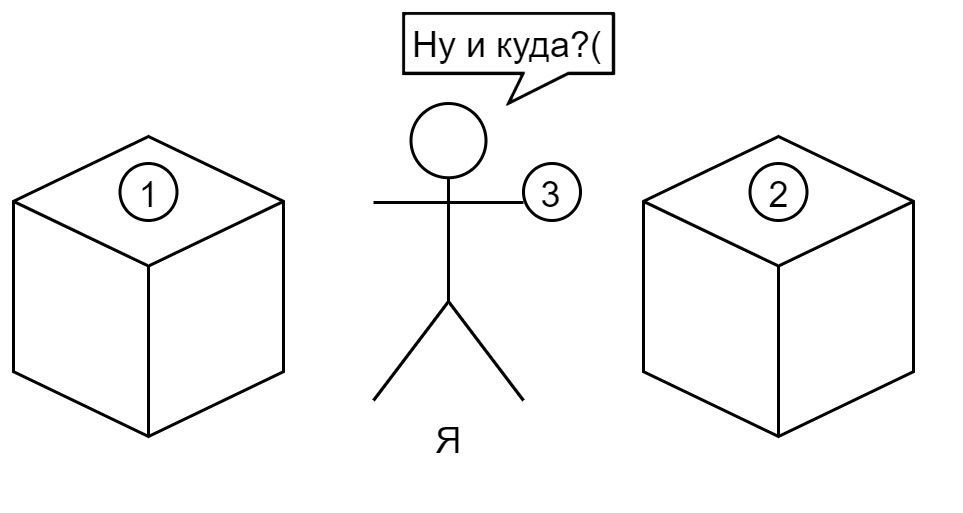
\includegraphics[scale=0.1]{b11.jpg}}
                \end{figure}\\
                \textit{Пример 2:} 1
                \begin{figure}[h!]
                    \fbox{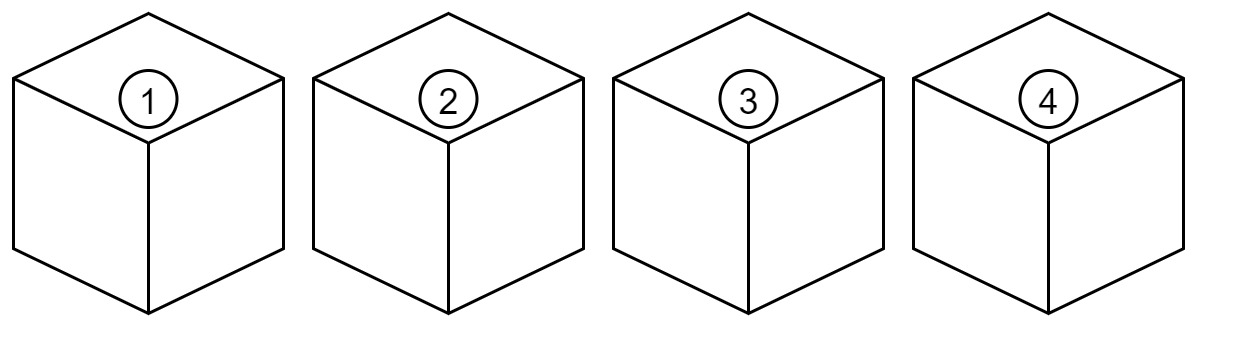
\includegraphics[scale=0.1]{b12.jpg}}
                \end{figure}
            \subsubsection{$\ge$ 1 мяч в коробке}
                Нам понадобится число Стирлинга второго рода, так как каждый из наших нумерованных шаров должен быть распределён по коробкам, следовательно:\\
                \textit{Общая формула:} $ S^{II}_{k}(n) $\\
                \textit{Пример 1:} $ S^{II}_{4}(5) = 10 $
                \begin{figure}[h!]
                    \fbox{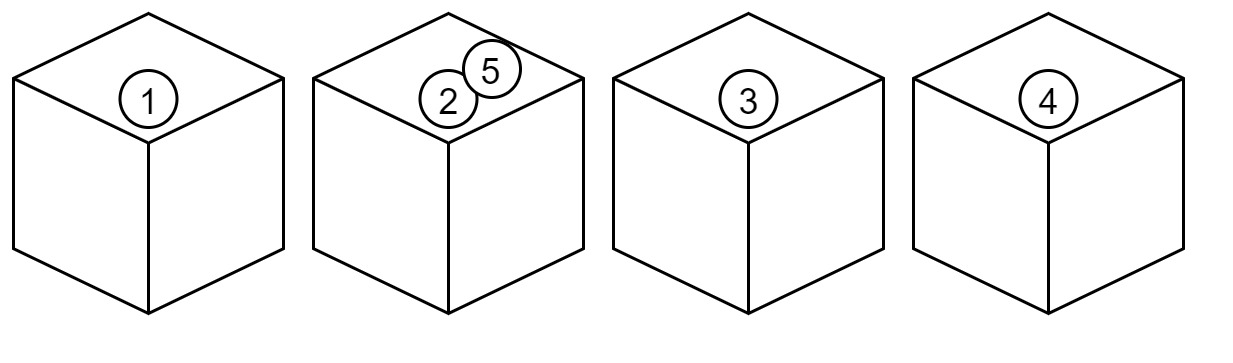
\includegraphics[scale=0.1]{b21.jpg}}
                \end{figure}\\
                \newpage
                \textit{Пример 2:} $ S^{II}_{4}(6) = 65 $
                \begin{figure}[h!]
                    \fbox{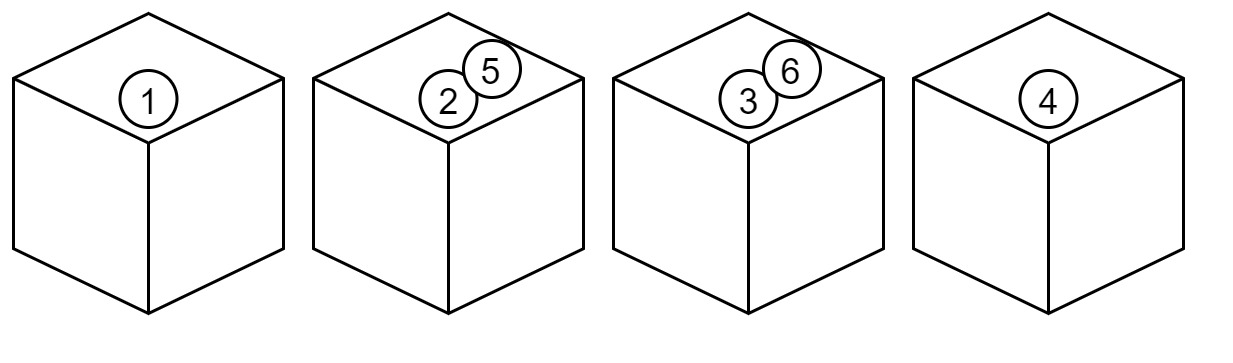
\includegraphics[scale=0.1]{b22.jpg}}
                \end{figure}
            \hypertarget{2b3}{\subsubsection{Произвольное количество шаров в коробке}}
                Нам нужна сумма числа Стирлинга второго рода, так как нужно распределить все нумерованные шары по коробкам, учитывая все варианты j-ого числа\\
                \textit{Общая формула:} $ \sum\limits_{j=1}^{k} S^{II}_{k}(n) $\\
                \textit{Пример 1:} $ \sum\limits_{j=1}^{4} S^{II}_{4}(5) = 52 $
                \begin{figure}[h!]
                    \fbox{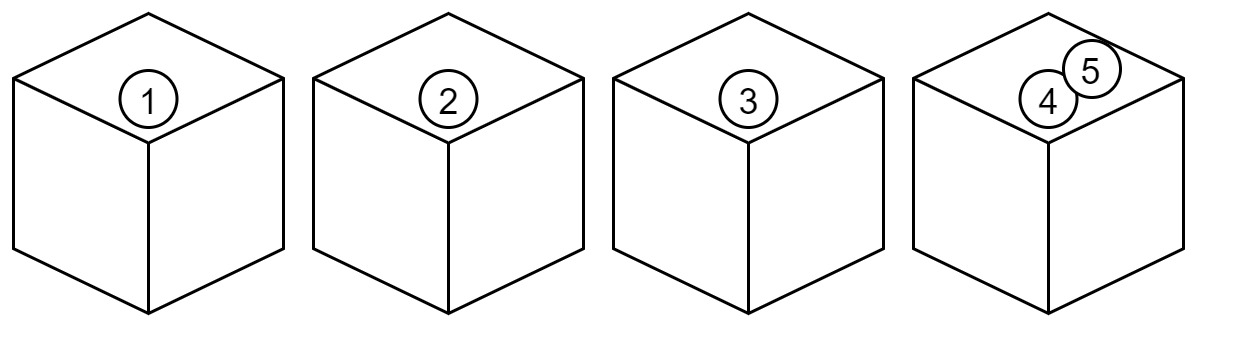
\includegraphics[scale=0.1]{b31.jpg}}
                \end{figure}\\
                \textit{Пример 2:} $ \sum\limits_{j=1}^{4} S^{II}_{4}(4) = 15 $
                \begin{figure}[h!]
                    \fbox{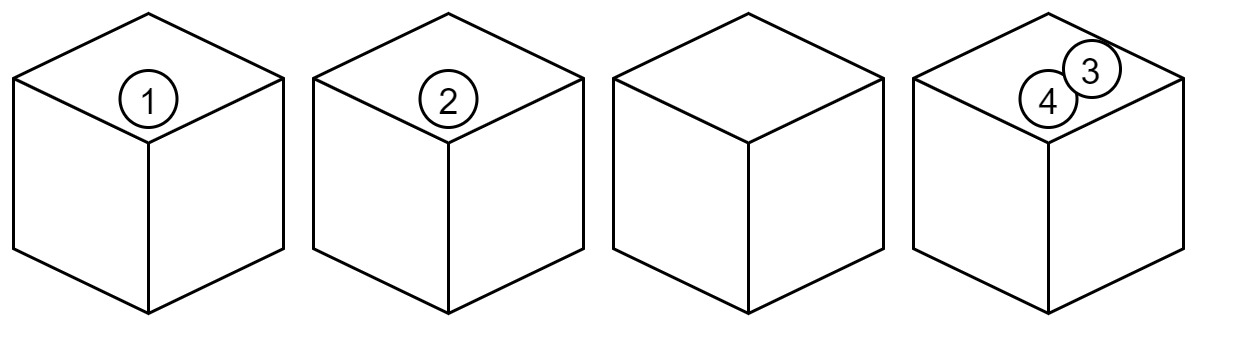
\includegraphics[scale=0.1]{b32.jpg}}
                \end{figure}
        \subsection{L → L: Шары помечены, Коробки помечены}
            \subsubsection{$\le$ 1 мяч на коробку}
                Так как нам нужно использовать все $n$ нумерованных шаров (не могут повторяться), то мы используем эту формулу:\\
                \textit{Общая формула:} $ A^n_k = \frac{k!}{(k-n)!} $\\
                \textit{Пример 1:} $ A^3_2 $ - невозможно, так как Шаров больше, чем Коробок - 0
                \begin{figure}[h!]
                    \fbox{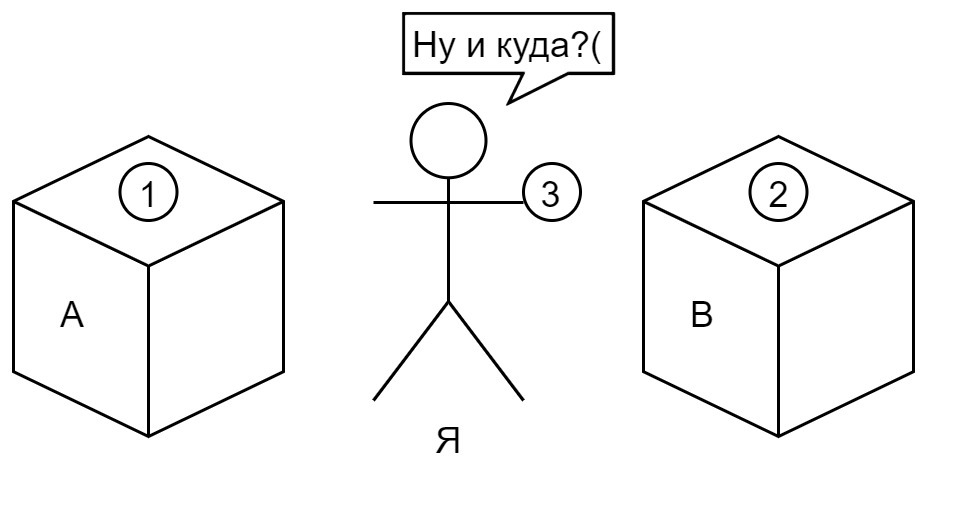
\includegraphics[scale=0.1]{c11.jpg}}
                \end{figure}\\
                \textit{Пример 2:} $ A^3_4 = 24 $
                \begin{figure}[h!]
                    \fbox{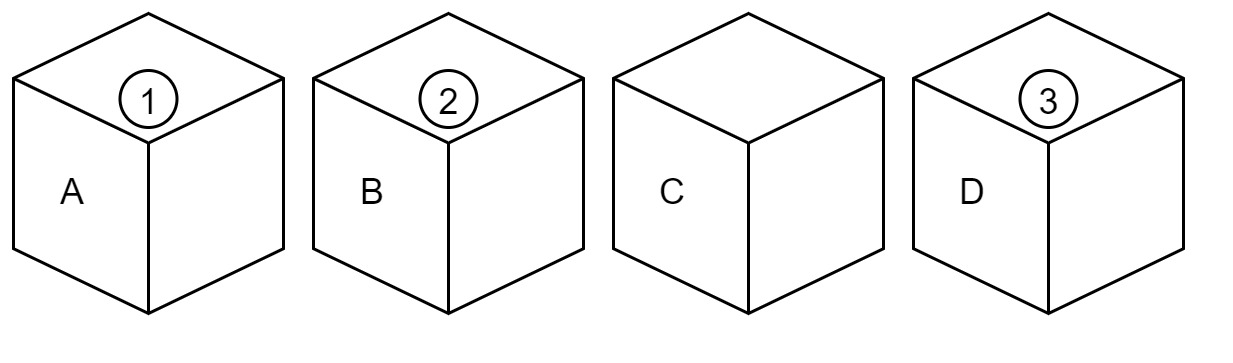
\includegraphics[scale=0.1]{с12.jpg}}
                \end{figure}
                \newpage
            \subsubsection{$\ge$ 1 мяч в коробке}
                Из-за того, что коробки нумерованны и шары тоже, то придётся использовать перестановки и число Стирлинга второго рода\\
                \textit{Общая формула:} $ S^{II}_{k}(n) * P_k = S^{II}_{k}(n) * k! $\\
                \textit{Пример 1:} $ S^{II}_{4}(5) * P_4  = 10*24 = 240 $
                \begin{figure}[h!]
                    \fbox{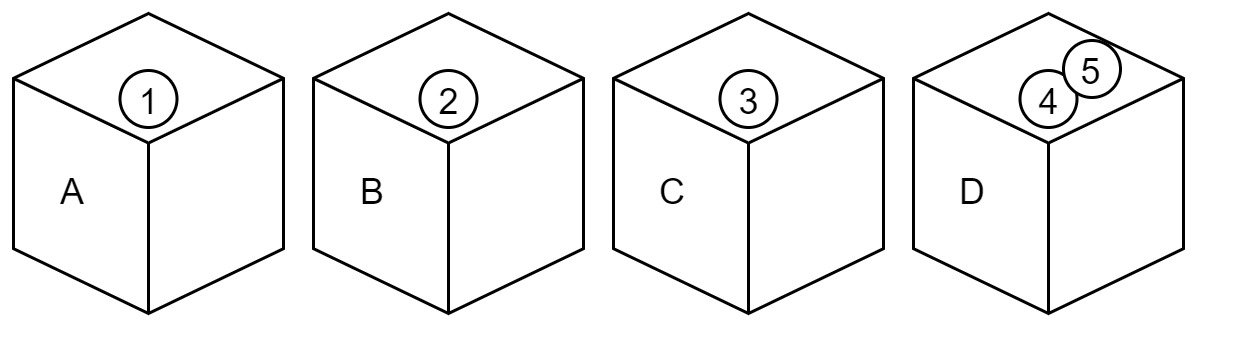
\includegraphics[scale=0.1]{с21.jpg}}
                \end{figure}\\
                \textit{Пример 2:} $ S^{II}_{4}(7) * P_4  = 350*24 = 8400 $
                \begin{figure}[h!]
                    \fbox{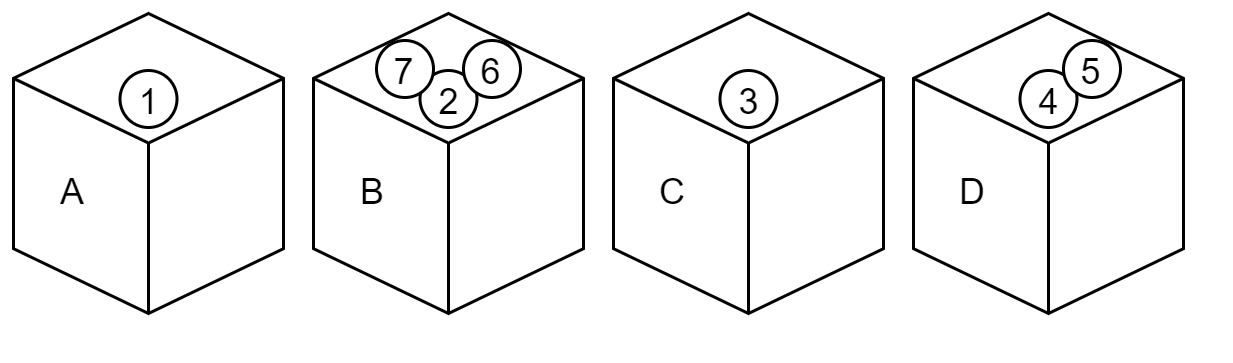
\includegraphics[scale=0.1]{с22.jpg}}
                \end{figure}
            \subsubsection{Произвольное количество шаров в коробке}
                Любой мяч может оказаться в любой коробке из-за произвольного количества шаров в коробке, следовательно:\\
                \textit{Общая формула:} $ \overline{A^n_k} = k^n $\\
                \textit{Пример 1:} $ \overline{A^6_4} = 4^6 = 4096 $
                \begin{figure}[h!]
                    \fbox{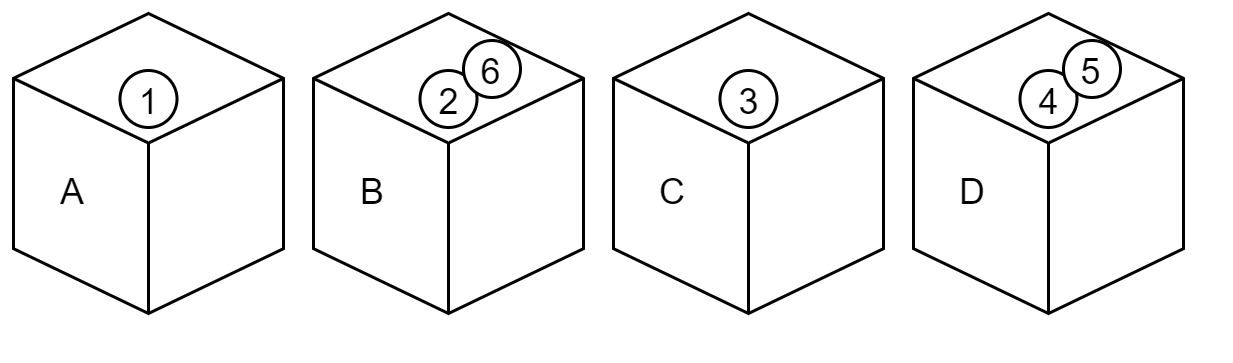
\includegraphics[scale=0.1]{с31.jpg}}
                \end{figure}\\
                \textit{Пример 2:} $ \overline{A^4_4} = 4^4 = 256 $
                \begin{figure}[h!]
                    \fbox{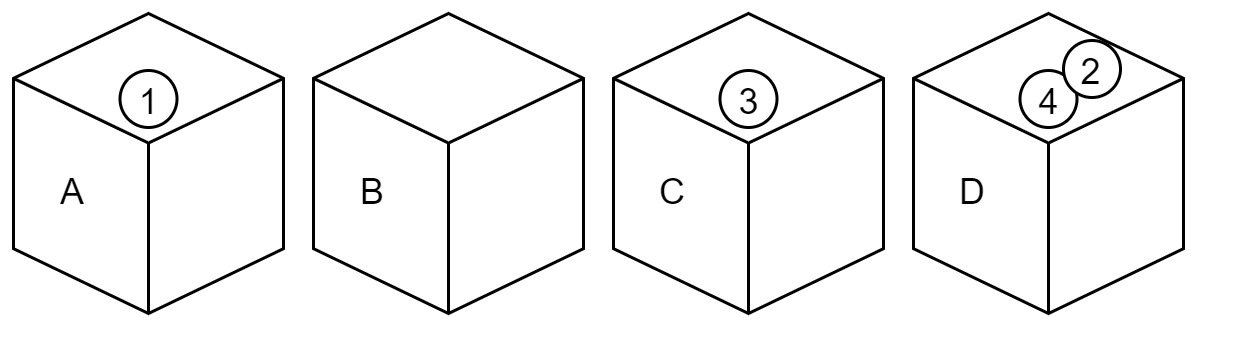
\includegraphics[scale=0.1]{с32.jpg}}
                \end{figure}
                %\newpage
        \subsection{U → U: Шары не помечены, Коробки не помечены}
            \subsubsection{$\le$ 1 мяч на коробку}
                Так как коробки неразличимы, то какие-то коробки пустые, а какие-то заполнены, следовательно - 1\\
                \textit{Пример 1:} Невозможно, так как Шаров больше, чем Коробок - 0
                \begin{figure}[h!]
                    \fbox{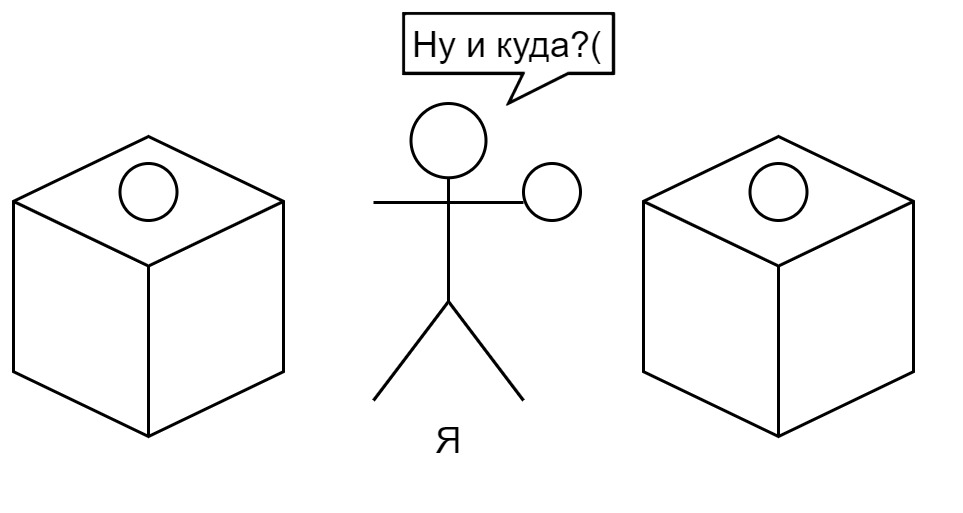
\includegraphics[scale=0.1]{d11.jpg}}
                \end{figure}\\
                \textit{Пример 2:} 1
                \begin{figure}[h!]
                    \fbox{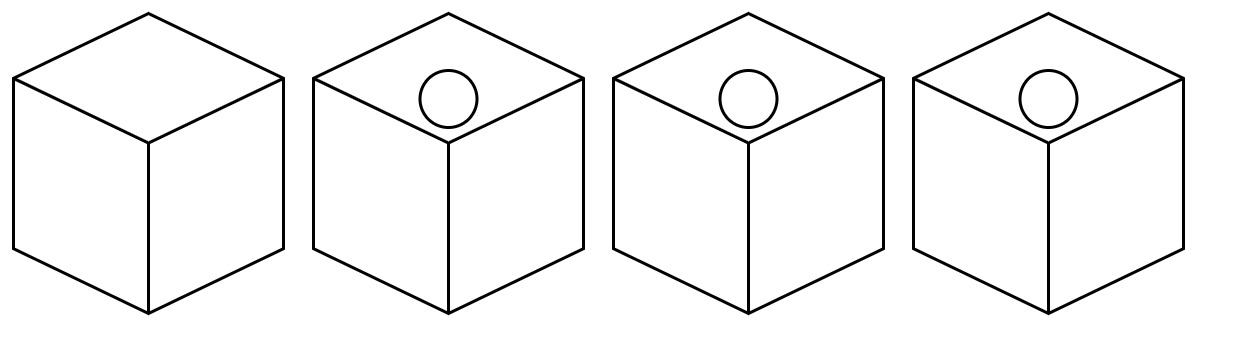
\includegraphics[scale=0.1]{d.jpg}}
                \end{figure}
            \subsubsection{$\ge$ 1 мяч в коробке}
                Из-за того, что у нас не пронумерованы ни Шары, ни Коробки, то придётся использовать разбиение числа:\\
                \textit{Общая формула:} $ p_k(n) $\\
                \textit{Пример 1:} $ p_4(5) = 1 $
                \begin{figure}[h!]
                    \fbox{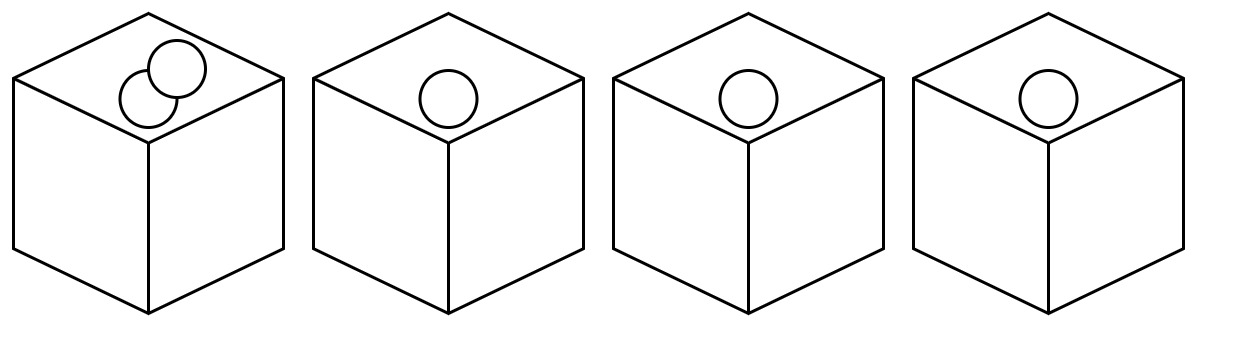
\includegraphics[scale=0.1]{d21.jpg}}
                \end{figure}\\
                \textit{Пример 2:} $ p_4(6) = 2 $
                \begin{figure}[h!]
                    \fbox{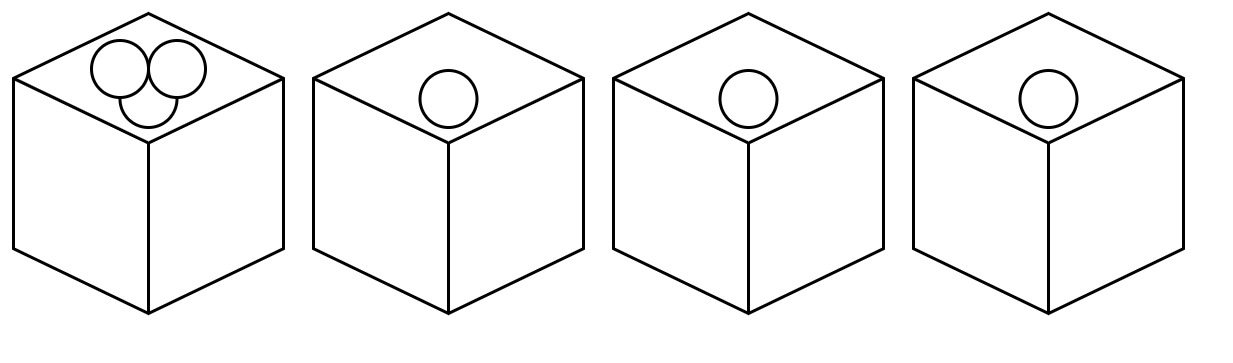
\includegraphics[scale=0.1]{d22.jpg}}
                \end{figure}
            \subsubsection{Произвольное количество шаров в коробке}
                Ситуация похожа на задание \hyperlink{2b3}{2.2.3}, только тут нам нужно использовать суммирование с разбиением числа, так как у нас ящики могут быть, как наполненными, так и пустыми и нужно учесть каждый из вариантов\\
                \textit{Общая формула:} $ \sum\limits_{j=1}^{k} p_j(n) $\\
                \textit{Пример 1:} $ \sum\limits_{j=1}^{4} p_j(6) = 1 + 3 + 2 + 2 = 8 $
                \begin{figure}[h!]
                    \fbox{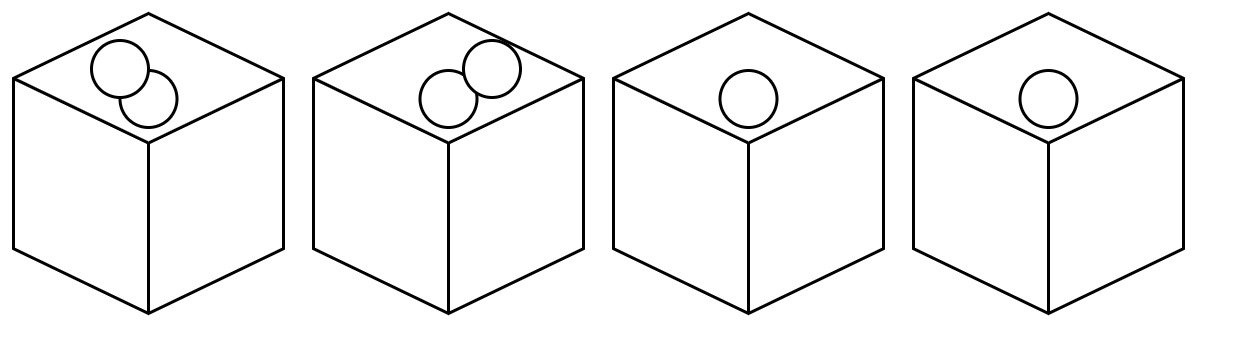
\includegraphics[scale=0.1]{d31.jpg}}
                \end{figure}\\
                \textit{Пример 2:} $ \sum\limits_{j=1}^{4} p_j(4) = 1 + 1 + 1 + 1 = 4 $
                \begin{figure}[h!]
                    \fbox{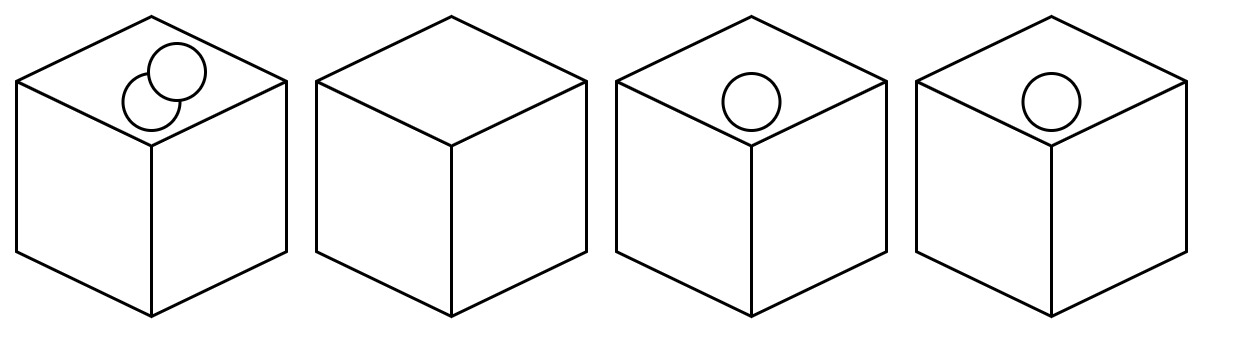
\includegraphics[scale=0.1]{d32.jpg}}
                \end{figure}
    \vfill
    \bigskip
    \small
    \begin{flushright}
        \href{https://ru.overleaf.com/read/nhnmvfbjzwhf}{Код отчёта на Overleaf}
    \end{flushright}
\end{document}